\chapter{No Camera}

\label{ch:no_camera}

\section{Design Choices}
\subsection{Radio Frequency Signal}


\subsubsection{Wi-Fi}

Wi-Fi is one of the most used Radio Frequency (RF) signals out there.
It is used for computer networking using 2.4 GHz UHF and 5 GHz SHF
ISM radio bands\cite{wifi-wikipedia}. The services provided are also
numerous, from consulting web pages to watching on demand video sequences. 

One of the biggest advantages of Wi-Fi is the fact that it\textquoteright s
widely used. Almost all location has Wi-Fi now, which means the setup
cost and maintenance cost of Wi-Fi would be cheap. It also has the
ability to transfer complicated data between its Access point (AP)
and the mobile devices, making it highly adaptable. 

Wi-Fi has been used for indoor positioning before by various research
groups. Two positioning techniques have been used for this research
called Signal Strength Cartography and Wave propagation. Signal Strength
Cartography is a reference-based system where you map the area offline
with coordinates and the strength of the Wi-Fi signal. Then when you
are trying to locate a device use the coordinates and the strength
to work out where exactly the device is. There are two main steps
for this mapping, an offline mapping step, which could be done either
by simulation or manually using measurements, and an online positioning
step, which could be done either using a probabilistic method or deterministic
method. 

Wave propagation approach is a mathematical attempt at finding the
distance between the device and the transmitter by finding a relation
between the distance and the signal strength. By using at least 3
AP we can use wave propagation and trilateration to work out the position
of the device. 

However there are various disadvantages of using Wi-Fi to work out
positioning of the devices. There are usually only one AP per location,
however we would require more than one, to get more accurate positioning
of the devices. Wi-Fi works mainly by sending signals in channels,
so having more than one Wi-Fi AP in a location could produce congestion
in channels, which would create interference. Wi-Fi also has a higher
power consumption. This is because of the larger range in which Wi-Fi
sends out its signal. 

There is hope for using Wi-Fi as the main Radio frequency for our
product in the future after the Wi-Fi Standards agency brings out
Wi-Fi -aware. Which is proximity based discovery system. Introduction
of this system could mean that you don\textquoteright t require any
extra AP, and the devices could interact with each other without any
outside help. 


\subsubsection{Global Positioning System (GPS)}

GPS is one of the most widely used features in our devices. Over the
past few years the use of GPS has increased significantly due to the
increasing social network activity. Nowadays almost every app that
we use through our mobile devices request for GPS access which shows
how much it has come forward. GPS is a space based navigation system
using the satellites. The Department of Defence of USA, using the
24 satellites already in orbit, initially introduced it. 

GPS satellites transmit data continuously, which contains their current
time and position. A GPS receiver listens to multiple satellites and
solves equations to determine the exact position of the receiver and
its deviation from true time. At a minimum, four satellites must be
in view of the receiver in order to compute four unknown quantities
(three position coordinates and clock deviation from satellite time). 

The main advantage of GPS is that it\textquoteright s widely available.
Almost all devices have a GPS receiver on it. It also has a very large
range. However it is not a viable option for us because of the fact
that the signal comes from outer space and our devices are usually
indoors. GPS like any radio frequency signal is prone to absorption
and diffraction by the roof and walls in the building. GPS also has
high power consumption. GPS tends to be not very accurate, averaging
\textasciitilde{}10m which would make it not feasible for our use. 


\subsubsection{Bluetooth}

Classic Bluetooth, usually known as Bluetooth, was the codename for
a project by Special Interest Group (SIG), collaboration between major
companies, like Ericsson, Intel, and Nokia. Bluetooth was invented
for short-range wireless communication with devices. Bluetooth uses
radio signals in the 2.4 GHz range to transmit data. This range is
globally license free range; therefore there is no extra cost for
deployment. Bluetooth is not targeted any specific application, therefore
a multitude of applications has used Bluetooth in various different
ways from transferring files to streaming songs.

SIG is in charge of the specification of Bluetooth and creating a
road map for it going forward. To standardise the form of communication
through Bluetooth, SIG has defined a set of profiles that needs to
be made available by the manufacturer. Devices usually only have a
subset of these profiles enabled. Some of these profiles are: 
\begin{itemize}
\item A2DP Advanced Audio Distribution Profile. Used for Streaming audio. 
\item HFP Hands-Free Profile. Used for hands free kit to make calls in cars 
\item HID Human Interface Device Profile. Provides support for input devices
like keyboards, mice and game controllers.
\end{itemize}
Bluetooth is aimed at applications that require short-range communication
typically few meters. The actual range an application make depends
on the Bluetooth Class the application has and also external circumstances
like absorption, diffraction etc. Bluetooth devices are separated
out into 3 different classes with separate transmission power. The
full picture is shown in Table 1.

\begin{tabular}{|c|c|c|c|}
\hline 
Class & Max Power Output & Max Range & Power Level Control\tabularnewline
\hline 
\hline 
1 & 100 mW & 100 m  & Mandatory\tabularnewline
\hline 
2 & 2.5 mW & 10 m & Optional\tabularnewline
\hline 
3 & 1 mW & 1 m & Optional\tabularnewline
\hline 
\end{tabular}
\begin{table}[H]
\protect\caption{Bluetooth Power class}
\end{table}


Due to the different profiles and more than sufficient range and relatively
low power consumption, Bluetooth shows considerable potential to be
used as our Radio frequency signal for our positioning. However they\textquoteright re
some aspects of it, which makes it difficult for Bluetooth to be used.
The main problem is the security constraints of Bluetooth, which requires
the devices to go through a pairing process with each other. 

In Bluetooth technology a device could take either the master role
or the slave role. Before the devices can communicate with each other
they have to discover each other and specify which profile they are
going to use. Pairing is done by: 
\begin{enumerate}
\item Master devices continuously broadcast \textquotedblleft inquiry messages\textquotedblright{}
\item These messages will be picked up by nearby devices that are \textquotedblleft discoverable\textquotedblright{} 
\item These devices will respond with a message containing their name, profiles
they support and other technical details. 
\item Using these details the master device can establish a connection with
the correct profile 
\end{enumerate}

\subsubsection{Bluetooth Low Energy (BLE)}

BLE is a relatively new technology, which came out in 2010 with the
new specification for Classic Bluetooth 4.0. BLE was introduced for
devices that are predominantly used for monitoring and control, like
sensors values and control commands, where there is no need for large
amount of data transfer.


\paragraph*{Modes\protect \\
}

One of the biggest improvements introduced for BLE that is not there
for Bluetooth is the addition of the new mode. This new mode takes
away the necessity for pairing to exchange data. In this \textquotedblleft broadcast\textquotedblright{}
mode the device can send data in the advertisement channel. There
are 4 different modes in BLE: 
\begin{description}
\item [{Central}] : Similar to the Bluetooth master role, can have multiple
connections. 
\item [{Peripheral:}] A device can only have one active connection with
the central mode 
\item [{Broadcaster}] : Where you send data in the advertisement channel
\item [{Observer:}] Where you listen to the advertisement channel
\end{description}

\paragraph*{Scanning\protect \linebreak{}
}

Another big improvement BLE has brought is the ability to discover
other devices in two different modes. BLE enabled devices can now
passively and actively scan for connectable devices.
\begin{itemize}
\item Passive scanning - a central device listens to the advertising channel
passively to capture all the packets transmitted by connectable devices 
\item Active scanning - a central device listen for advertisement packets
and when it receives the packet, it checks whether the sender is connectable
through looking at the mode. If it is then a scan request packet is
send to gain more information.
\end{itemize}
Devices may advertise as seldom as once every 10 seconds or as fast
as every 20 millisecond. 


\paragraph*{Range\protect \\
}

Similar to the Classic Bluetooth, the range of BLE is determined by
the transmitting power and the interference that it might experience.
BLE has a transmitting power up +10dBm, which gives it a range of
300m theoretically. However BLE usually use a power of 0dB or less
which gives it a range of about 50m. Even though BLE is meant to have
low-energy consumption, it has a bigger range than Classic Bluetooth
under maximum power due to smaller packet size. 


\subsection{Others eg Zigbee}

There are various other technology out there that could be used such
as Zigbee. However since these are not commonly supported by mobile
devices. Therefore they have not been considered for the implementation.

\subsection{Positioning algorithms}


\subsubsection{Ecolocation}

Ecolocation\cite{Ecolocation} is a technique which uses RF and distance
to work out the location of a node in a Wireless Sensor Network (WSN).
They use sense and match system, where the unknown node listens for
packets from all the reference nodes. It orders the packets in the
distance it has traveled, and then try and match it to known distance
orders. 

In an ideal scenario the Relative Signal Strength (RSS) reading from
each reference node would be an accurate indication of the distance
between the nodes. By ranking the sequence of RSS readings we can
find a constrain on the location of the unknown node. By having multiple
reference nodes we are increasing the constraints to find the unknown
node. By having fixed reference node locations and the sequence order
of the RSS reading and the constraints are determined by the unknown
node location. The unknown node location estimate can be obtained
by comparing the constraints obtained from RSS measurements to the
constraint sets of each location grid-point and picking the location
which satisfies the maximum number of constraints. If there are more
than one such locations then their centroid is the location estimate.

However in a real world presence of multi-path fading and shadowing
in the RF channel impacts the RSS reading greatly. We would assume
that reference nodes that are far from the unknown node should measure
lower RSS values than the nodes that are near to it. However due to
multi-path fading this is not always true. The percentage of error
depends on the RF channel condition and the topology and the number
of reference nodes. Tests show that Ecolocation is robust to multi-path
effects of RF channel to some degree. The technique can eradicate
the errors due to random variation in RSS measurements up to a tolerance
level of |R\textsubscript{i}-R\textsubscript{j}| due to the way
its constructed.

Experimental results done by Yedavalli, K. and Krishnamachari, B.
et all shows that localization techniques are more accurate for relatively
clutter free RF channel environments i.e outdoors with a clear line
of sight. Their research also concluded that a single localization
methods does not provide sufficient accuracy for all their unknown
nodes, they recommend a hybrid localization techniques depending the
RF channel and node deployment parameters would proved a better accuracy.
They have also not taken any complexity into account, using Ecolocation
would require a large amount of ``offline'' work where you would
have to go through different locations in the space to calculate the
RSS readings at that location and save those readings. This would
be a resource intensive and time consuming operation making it not
ideal in a system mainly targeting mobile devices.


\subsubsection{Trilateration}

Trilateration is the process of finding an absolute point or a relative
point of an object using measured distances between the object and
multiple reference points. Trilateration works by finding the intersection
of three circles centered at anchor as the position of the node. The
general equation of a sphere is :
\[
d^{2}=x^{2}+y^{2}+z^{2}
\]


For a sphere centered at a point (x\textsubscript{a} , y\textsubscript{a}
, z\textsubscript{a}) where x$_{a}$is at the origin and x$_{b}$is
the x coordinate of d$_{b}$ the equation is simplified as:

\begin{figure}[H]
\[
d_{a}^{2}=x^{2}+y^{2}+z^{2}
\]


\[
d_{b}^{2}=\left(x-x_{b}\right)^{2}+y^{2}+z^{2}
\]


\[
d_{c}^{2}=\left(x-x_{c}\right)^{2}+\left(y-y_{c}\right)^{2}+\left(z-z_{c}\right)^{2}
\]


\protect\caption{Equation of 3 spheres}


\end{figure}


We need to find a position (x, y, z) that satisfies all three equations.
We can use d$_{a}$ and d$_{b}$ to eliminate y and z from the equation
so that we can solve for x. i.e.

\begin{figure}[H]
\[
d_{a}^{2}-d_{b}^{2}=x^{2}-\left(x-x_{b}\right)^{2}
\]


\[
d_{a}^{2}-d_{b}^{2}=x^{2}-\left(x^{2}-2xx_{b}+d^{2}\right)
\]


\[
d_{a}^{2}-d_{b}^{2}=2xx_{b}-d^{2}
\]


\[
x=\frac{d_{a}^{2}-d_{b}^{2}+d^{2}}{2x_{b}}
\]


\protect\caption{Derivation to get x}
\end{figure}


Assuming that the two spheres intersect at more than 1 point, then 

\[
x_{a}-d_{a}<d_{b}<d_{a}+x_{a}
\]


\begin{figure}[H]
\protect\caption{Substituting to get y and z}


\end{figure}


It is a widely used and one of the most popular method for finding
a location of an unknown devices. It is one of the main component
of the Global Positioning System (GPS), which uses the time taken
for the signal to travel from 4 satellites to our mobile devices,
to work out the location of the device.

\_\_\_\_\_ 


\subsubsection{Inertial Navigation System (INS)}

INS \_\_\_\_\_ is based on the internal sensors that a devices have
such as Accelerometer, Gyroscope etc. We can use the information from
these sensors to keep track of the position and the orientation of
the mobile device relative to the starting position and orientation
of the device. INS has many uses, including navigation systems for
aircraft and missiles.


\paragraph{Accelerometer}

Accelerometer is a very common sensors that are built into almost
all the mobile devices out there. It measures the proper acceleration
of the device which might not be the same as the coordinate acceleration
(change in velocity over time). Proper acceleration is the weight
experienced by a test mass that which is in the frame of reference
of the accelerometer device. So accelerometer measure how much mass
presses on something when a force acts on it.

Any accelerometer at rest on a surface will show an acceleration of
approximately 1G upwards, due to the earths gravitational force. At
any point on earths surface there is an acceleration of 1G upwards
relative to the local frame. This offset has to be subtracted to get
the motion with respect to the Earth. There are many uses for accelerometer,
monitoring vibrations and they are also used in mobile devices to
keep the images displayed on the screen upright. Highly sensitive
accelerometers are used in drones for flight stabilisation.

Mobile devices are usually equipped with a multi-axis models of accelerometers
so that they can detect magnitude and direction of acceleration as
vector quantity. They can then we used to work out the displacement
of a device. However the accelerometers used by the android devices
are not very accurate, therefore there is a lot of noise and calibration
steps required before hand by the user to get a acceptable results.

\begin{figure}[H]
\[
x=\int\int a\mathrm{\text{ }d}t
\]
 

\protect\caption{Acceleration to displacement}


\end{figure}



\paragraph{Gyroscope}

Gyroscope is a device for measuring and determining the orientation
of a device. This is done be using the principles of conservation
of angular momentum. A gyroscope usually consist of a free rotating
disk called a rotor mounted on a spinning axes, in center of a large
more stable wheel, which lets it rotate in all the axes. As the axis
turns, the rotor remains stationary to indicate the central gravitational
pull, therefore showing us which way is down.

One of the best examples of reading a gyroscope is the altitude indicator
of an aircraft. It is represented by a circular display divided in
half. The top half is blue indicating the sky and the bottom half
is red to show the ground. As the aircraft banks for a turn, the indicator
with shift to account for the actual direction of the ground.

Gyroscopes are also used in INS. Another advantage of them are, that
you can use them where magnetic compasses don't work such as the Huddle
Telescope\cite{gyroscope-wiki}.


\subsubsection{Filter Methods}


\paragraph{Kalman Filter}




\subsection{Beacon Vendors}

I have decided to use the iBeacon technology pioneered by Apple as
the underlying technology for my project. Beekn\cite{beekn} is a
website that has accumulated a lot of information about iBeacons.
As they have reviewed there a lot of vendors who provide good iBeacon
technology. In this section I will look at the main vendors I have
considered and also the Intel Gallileo chip which is a more powerful
chip.


\subsubsection{Qualcomm}

Qualcomm\cite{quallcomm} is one of the biggest chip manufacturing
companies. They are a world leader in 3G and next generation mobile
technologies. Naturally they have also launched their brand of beacons
called Gimbal\cite{gimbal}. The Gimbal beacons are relatively cheap
around \$5 when bought in bulk. However the main advantage is the
robust back-end system and SDK. Gimbal is launched in 2 sizes:

\begin{figure}[H]
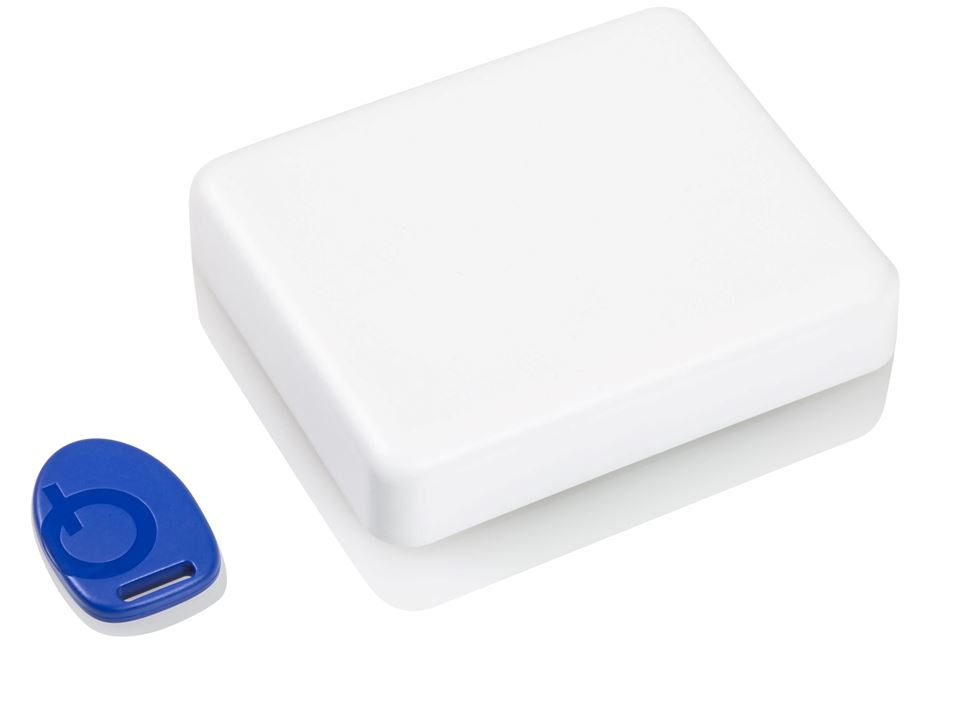
\includegraphics[scale=0.3]{images/gimbal-beacon}

\protect\caption{Gimbal Beacons}
\end{figure}

\begin{enumerate}
\item Series 10: Comes in a small size, (28mmx40mmx5.6mm), and comes with
a loop to allow installation flexibility. The battery life is around
3 months and transmission rate of twice per second. It also has a
temperature sensor on it.
\item Series 20: Comes in a bigger size, size of a playing card. It is also
more robust than the series 10. It uses replaceable AA alkaline battery
giving it more battery life and also a higher transmitting rate.
\end{enumerate}
More than the size and robustness of the beacons, the factor that
sets Gimbal apart from its competitors is its back-end system. Gimbal
is shipped with a full functioning back-end system that supports Geo-fencing\cite{geofencing},
analytic, communication tools and application management. They have
also introduced features such as allowing developers to set up rules
for entering and exiting the beacon proximity.


\subsubsection{Estimote}

Estimote\cite{estimote} is an upcoming start up that has made waves
in the beacon technology market. Having sold over 40,000 developer
kits since its launch in 2013, it is one of the biggest company for
beacons enjoying a large market share. Similar to the Gimbal they
also launch in 2 Sizes. However the Estimote beacons are relatively
more expensive than the Gimbal.
\begin{enumerate}
\item The main product is called Estimote Beacon which is quite a large
product. It's main role, is to be stationary stuck onto a wall somewhere
i.e in a supermarket, for Geo-fence it to give targeted advertisement
to the users depending on the location.  
\item They have also recently brought out another product called Estimote
Stickers. Which is more like a rival to the Gimbal series 10, its
a smaller version of the beacon which can potentially turn any device
into a nearable. It also has sensors in it such as accelerometer and
temperature to give a more detailed information on the activity and
the location of the device its stuck onto.
\begin{figure}[H]
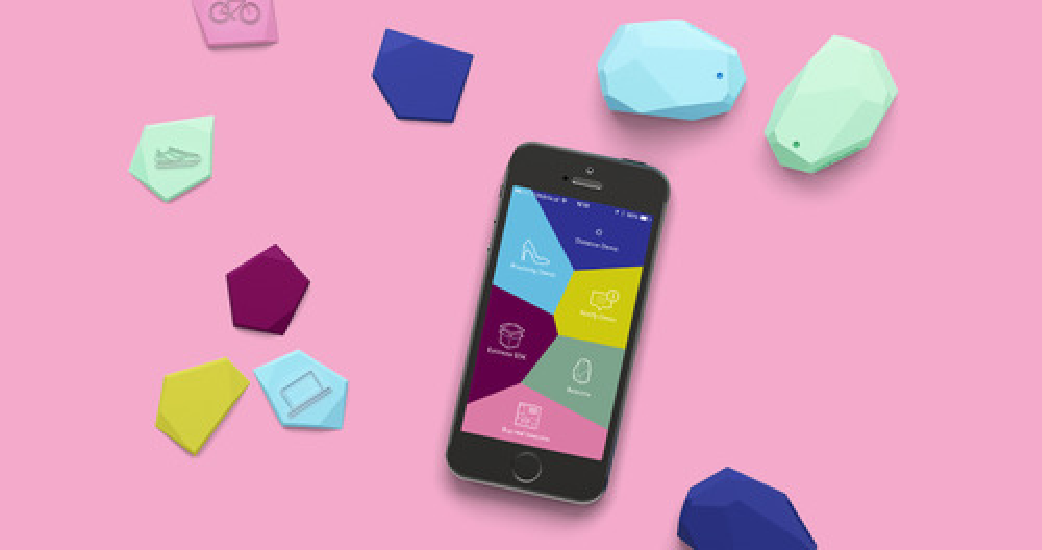
\includegraphics[scale=0.3]{images/estimote}

\protect\caption{Estimote beacons}


\end{figure}

\end{enumerate}

\subsubsection{Intel Edison}

Intel Edison\cite{intel-edision} is a tiny computer offered by Intel
as a development system for wearable devices. It has a high performance
dual core CPU with integrated Wi-Fi and BLE, all using very low battery.
Making it have all the capabilities of a computer with a longer battery
life and more portability. It is one of the main components used in
Internet of Things (IoT). It has access to device-to-device and device-to-cloud
connectivity framework to enable cross device communication and a
cloud based, multi-tenant, time-series analytic service. Since it
is a highly powerful machine with both Wi-fi and BLE support, its
an ideal candidate for the beacons I need for my research. However
due to its relatively low battery life (around 1 day) and it having
more power and facilities than I need, I have not used the Edison.

\begin{figure}[H]
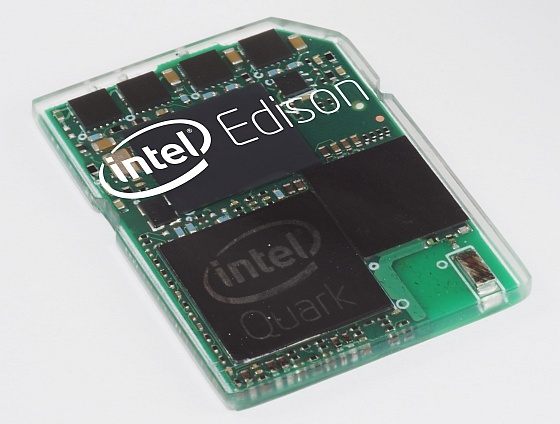
\includegraphics{images/intel-edison-560}

\protect\caption{Intel Edison}


\end{figure}


